\documentclass[1p]{elsarticle_modified}
%\bibliographystyle{elsarticle-num}

%\usepackage[colorlinks]{hyperref}
%\usepackage{abbrmath_seonhwa} %\Abb, \Ascr, \Acal ,\Abf, \Afrak
\usepackage{amsfonts}
\usepackage{amssymb}
\usepackage{amsmath}
\usepackage{amsthm}
\usepackage{scalefnt}
\usepackage{amsbsy}
\usepackage{kotex}
\usepackage{caption}
\usepackage{subfig}
\usepackage{color}
\usepackage{graphicx}
\usepackage{xcolor} %% white, black, red, green, blue, cyan, magenta, yellow
\usepackage{float}
\usepackage{setspace}
\usepackage{hyperref}

\usepackage{tikz}
\usetikzlibrary{arrows}

\usepackage{multirow}
\usepackage{array} % fixed length table
\usepackage{hhline}

%%%%%%%%%%%%%%%%%%%%%
\makeatletter
\renewcommand*\env@matrix[1][\arraystretch]{%
	\edef\arraystretch{#1}%
	\hskip -\arraycolsep
	\let\@ifnextchar\new@ifnextchar
	\array{*\c@MaxMatrixCols c}}
\makeatother %https://tex.stackexchange.com/questions/14071/how-can-i-increase-the-line-spacing-in-a-matrix
%%%%%%%%%%%%%%%

\usepackage[normalem]{ulem}

\newcommand{\msout}[1]{\ifmmode\text{\sout{\ensuremath{#1}}}\else\sout{#1}\fi}
%SOURCE: \msout is \stkout macro in https://tex.stackexchange.com/questions/20609/strikeout-in-math-mode

\newcommand{\cancel}[1]{
	\ifmmode
	{\color{red}\msout{#1}}
	\else
	{\color{red}\sout{#1}}
	\fi
}

\newcommand{\add}[1]{
	{\color{blue}\uwave{#1}}
}

\newcommand{\replace}[2]{
	\ifmmode
	{\color{red}\msout{#1}}{\color{blue}\uwave{#2}}
	\else
	{\color{red}\sout{#1}}{\color{blue}\uwave{#2}}
	\fi
}

\newcommand{\Sol}{\mathcal{S}} %segment
\newcommand{\D}{D} %diagram
\newcommand{\A}{\mathcal{A}} %arc


%%%%%%%%%%%%%%%%%%%%%%%%%%%%%5 test

\def\sl{\operatorname{\textup{SL}}(2,\Cbb)}
\def\psl{\operatorname{\textup{PSL}}(2,\Cbb)}
\def\quan{\mkern 1mu \triangleright \mkern 1mu}

\theoremstyle{definition}
\newtheorem{thm}{Theorem}[section]
\newtheorem{prop}[thm]{Proposition}
\newtheorem{lem}[thm]{Lemma}
\newtheorem{ques}[thm]{Question}
\newtheorem{cor}[thm]{Corollary}
\newtheorem{defn}[thm]{Definition}
\newtheorem{exam}[thm]{Example}
\newtheorem{rmk}[thm]{Remark}
\newtheorem{alg}[thm]{Algorithm}

\newcommand{\I}{\sqrt{-1}}
\begin{document}

%\begin{frontmatter}
%
%\title{Boundary parabolic representations of knots up to 8 crossings}
%
%%% Group authors per affiliation:
%\author{Yunhi Cho} 
%\address{Department of Mathematics, University of Seoul, Seoul, Korea}
%\ead{yhcho@uos.ac.kr}
%
%
%\author{Seonhwa Kim} %\fnref{s_kim}}
%\address{Center for Geometry and Physics, Institute for Basic Science, Pohang, 37673, Korea}
%\ead{ryeona17@ibs.re.kr}
%
%\author{Hyuk Kim}
%\address{Department of Mathematical Sciences, Seoul National University, Seoul 08826, Korea}
%\ead{hyukkim@snu.ac.kr}
%
%\author{Seokbeom Yoon}
%\address{Department of Mathematical Sciences, Seoul National University, Seoul, 08826,  Korea}
%\ead{sbyoon15@snu.ac.kr}
%
%\begin{abstract}
%We find all boundary parabolic representation of knots up to 8 crossings.
%
%\end{abstract}
%\begin{keyword}
%    \MSC[2010] 57M25 
%\end{keyword}
%
%\end{frontmatter}

%\linenumbers
%\tableofcontents
%
\newcommand\colored[1]{\textcolor{white}{\rule[-0.35ex]{0.8em}{1.4ex}}\kern-0.8em\color{red} #1}%
%\newcommand\colored[1]{\textcolor{white}{ #1}\kern-2.17ex	\textcolor{white}{ #1}\kern-1.81ex	\textcolor{white}{ #1}\kern-2.15ex\color{red}#1	}

{\Large $\underline{12n_{0501}~(K12n_{0501})}$}

\setlength{\tabcolsep}{10pt}
\renewcommand{\arraystretch}{1.6}
\vspace{1cm}\begin{tabular}{m{100pt}>{\centering\arraybackslash}m{274pt}}
\multirow{5}{120pt}{
	\centering
	\includegraphics[width=112pt]{../../../GIT/diagram.site/Diagrams/png/2590_12n_0501.png}\\
\ \ \ A knot diagram\footnotemark}&
\allowdisplaybreaks
\textbf{Linearized knot diagam} \\
\cline{2-2}
 &
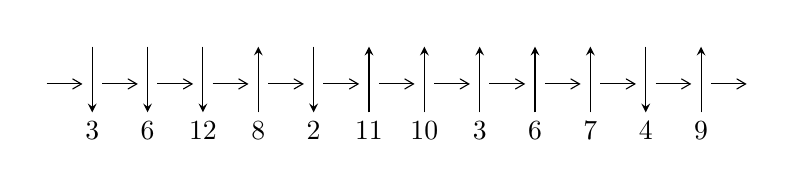
\begin{tikzpicture}[x=20pt, y=17pt]
	% nodes
	\node (C0) at (0, 0) {};
	\node (C1) at (1, 0) {};
	\node (C1U) at (1, +1) {};
	\node (C1D) at (1, -1) {3};

	\node (C2) at (2, 0) {};
	\node (C2U) at (2, +1) {};
	\node (C2D) at (2, -1) {6};

	\node (C3) at (3, 0) {};
	\node (C3U) at (3, +1) {};
	\node (C3D) at (3, -1) {12};

	\node (C4) at (4, 0) {};
	\node (C4U) at (4, +1) {};
	\node (C4D) at (4, -1) {8};

	\node (C5) at (5, 0) {};
	\node (C5U) at (5, +1) {};
	\node (C5D) at (5, -1) {2};

	\node (C6) at (6, 0) {};
	\node (C6U) at (6, +1) {};
	\node (C6D) at (6, -1) {11};

	\node (C7) at (7, 0) {};
	\node (C7U) at (7, +1) {};
	\node (C7D) at (7, -1) {10};

	\node (C8) at (8, 0) {};
	\node (C8U) at (8, +1) {};
	\node (C8D) at (8, -1) {3};

	\node (C9) at (9, 0) {};
	\node (C9U) at (9, +1) {};
	\node (C9D) at (9, -1) {6};

	\node (C10) at (10, 0) {};
	\node (C10U) at (10, +1) {};
	\node (C10D) at (10, -1) {7};

	\node (C11) at (11, 0) {};
	\node (C11U) at (11, +1) {};
	\node (C11D) at (11, -1) {4};

	\node (C12) at (12, 0) {};
	\node (C12U) at (12, +1) {};
	\node (C12D) at (12, -1) {9};
	\node (C13) at (13, 0) {};

	% arrows
	\draw[->,>={angle 60}]
	(C0) edge (C1) (C1) edge (C2) (C2) edge (C3) (C3) edge (C4) (C4) edge (C5) (C5) edge (C6) (C6) edge (C7) (C7) edge (C8) (C8) edge (C9) (C9) edge (C10) (C10) edge (C11) (C11) edge (C12) (C12) edge (C13) ;	\draw[->,>=stealth]
	(C1U) edge (C1D) (C2U) edge (C2D) (C3U) edge (C3D) (C4D) edge (C4U) (C5U) edge (C5D) (C6D) edge (C6U) (C7D) edge (C7U) (C8D) edge (C8U) (C9D) edge (C9U) (C10D) edge (C10U) (C11U) edge (C11D) (C12D) edge (C12U) ;
	\end{tikzpicture} \\
\hhline{~~} \\& 
\textbf{Solving Sequence} \\ \cline{2-2} 
 &
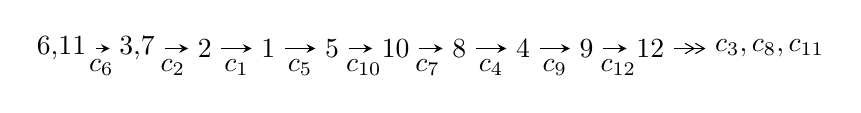
\begin{tikzpicture}[x=23pt, y=7pt]
	% node
	\node (A0) at (-1/8, 0) {6,11};
	\node (A1) at (17/16, 0) {3,7};
	\node (A2) at (17/8, 0) {2};
	\node (A3) at (25/8, 0) {1};
	\node (A4) at (33/8, 0) {5};
	\node (A5) at (41/8, 0) {10};
	\node (A6) at (49/8, 0) {8};
	\node (A7) at (57/8, 0) {4};
	\node (A8) at (65/8, 0) {9};
	\node (A9) at (73/8, 0) {12};
	\node (C1) at (1/2, -1) {$c_{6}$};
	\node (C2) at (13/8, -1) {$c_{2}$};
	\node (C3) at (21/8, -1) {$c_{1}$};
	\node (C4) at (29/8, -1) {$c_{5}$};
	\node (C5) at (37/8, -1) {$c_{10}$};
	\node (C6) at (45/8, -1) {$c_{7}$};
	\node (C7) at (53/8, -1) {$c_{4}$};
	\node (C8) at (61/8, -1) {$c_{9}$};
	\node (C9) at (69/8, -1) {$c_{12}$};
	\node (A10) at (11, 0) {$c_{3},c_{8},c_{11}$};

	% edge
	\draw[->,>=stealth]	
	(A0) edge (A1) (A1) edge (A2) (A2) edge (A3) (A3) edge (A4) (A4) edge (A5) (A5) edge (A6) (A6) edge (A7) (A7) edge (A8) (A8) edge (A9) ;
	\draw[->>,>={angle 60}]	
	(A9) edge (A10);
\end{tikzpicture} \\ 

\end{tabular} \\

\footnotetext{
The image of knot diagram is generated by the software ``\textbf{Draw programme}" developed by Andrew Bartholomew(\url{http://www.layer8.co.uk/maths/draw/index.htm\#Running-draw}), where we modified some parts for our purpose(\url{https://github.com/CATsTAILs/LinksPainter}).
}\phantom \\ \newline 
\centering \textbf{Ideals for irreducible components\footnotemark of $X_{\text{par}}$} 
 
\begin{align*}
I^u_{1}&=\langle 
-4 u^{32}+16 u^{31}+\cdots+4 b+5,\;5 u^{32}-16 u^{31}+\cdots+4 a+6,\;u^{33}-4 u^{32}+\cdots-6 u+1\rangle \\
I^u_{2}&=\langle 
- a u+b,\;2 u^2 a+a^2+a u+2 u^2+3 a+u+4,\;u^3+u^2+2 u+1\rangle \\
I^u_{3}&=\langle 
u^2+b+u+1,\;- u^2+a-1,\;u^3+u^2+2 u+1\rangle \\
\\
\end{align*}
\raggedright * 3 irreducible components of $\dim_{\mathbb{C}}=0$, with total 42 representations.\\
\footnotetext{All coefficients of polynomials are rational numbers. But the coefficients are sometimes approximated in decimal forms when there is not enough margin.}
\newpage
\renewcommand{\arraystretch}{1}
\centering \section*{I. $I^u_{1}= \langle -4 u^{32}+16 u^{31}+\cdots+4 b+5,\;5 u^{32}-16 u^{31}+\cdots+4 a+6,\;u^{33}-4 u^{32}+\cdots-6 u+1 \rangle$}
\flushleft \textbf{(i) Arc colorings}\\
\begin{tabular}{m{7pt} m{180pt} m{7pt} m{180pt} }
\flushright $a_{6}=$&$\begin{pmatrix}1\\0\end{pmatrix}$ \\
\flushright $a_{11}=$&$\begin{pmatrix}0\\u\end{pmatrix}$ \\
\flushright $a_{3}=$&$\begin{pmatrix}-\frac{5}{4} u^{32}+4 u^{31}+\cdots+\frac{7}{4} u-\frac{3}{2}\\u^{32}-4 u^{31}+\cdots+9 u-\frac{5}{4}\end{pmatrix}$ \\
\flushright $a_{7}=$&$\begin{pmatrix}1\\- u^2\end{pmatrix}$ \\
\flushright $a_{2}=$&$\begin{pmatrix}-\frac{1}{4} u^{32}-\frac{5}{2} u^{30}+\cdots+\frac{43}{4} u-\frac{11}{4}\\u^{32}-4 u^{31}+\cdots+9 u-\frac{5}{4}\end{pmatrix}$ \\
\flushright $a_{1}=$&$\begin{pmatrix}-\frac{11}{4} u^{32}+\frac{41}{4} u^{31}+\cdots-23 u+\frac{11}{2}\\\frac{3}{4} u^{32}-3 u^{31}+\cdots+\frac{63}{4} u-\frac{15}{4}\end{pmatrix}$ \\
\flushright $a_{5}=$&$\begin{pmatrix}-\frac{1}{4} u^{32}+\frac{3}{4} u^{31}+\cdots-4 u+\frac{1}{4}\\\frac{1}{4} u^{32}- u^{31}+\cdots+\frac{13}{4} u-\frac{1}{2}\end{pmatrix}$ \\
\flushright $a_{10}=$&$\begin{pmatrix}- u\\u^3+u\end{pmatrix}$ \\
\flushright $a_{8}=$&$\begin{pmatrix}u^2+1\\- u^4-2 u^2\end{pmatrix}$ \\
\flushright $a_{4}=$&$\begin{pmatrix}-\frac{1}{2} u^{32}+\frac{7}{4} u^{31}+\cdots-\frac{29}{4} u+\frac{3}{4}\\\frac{1}{4} u^{32}- u^{31}+\cdots+\frac{17}{4} u-\frac{3}{4}\end{pmatrix}$ \\
\flushright $a_{9}=$&$\begin{pmatrix}- u^3-2 u\\u^3+u\end{pmatrix}$ \\
\flushright $a_{12}=$&$\begin{pmatrix}-\frac{9}{4} u^{32}+\frac{33}{4} u^{31}+\cdots-\frac{37}{2} u+\frac{19}{4}\\\frac{3}{4} u^{32}-\frac{11}{4} u^{31}+\cdots+13 u-\frac{13}{4}\end{pmatrix}$\\&\end{tabular}
\flushleft \textbf{(ii) Obstruction class $= -1$}\\~\\
\flushleft \textbf{(iii) Cusp Shapes $= -\frac{9}{2} u^{32}+\frac{35}{2} u^{31}+\cdots-\frac{111}{2} u+\frac{23}{4}$}\\~\\
\newpage\renewcommand{\arraystretch}{1}
\flushleft \textbf{(iv) u-Polynomials at the component}\newline \\
\begin{tabular}{m{50pt}|m{274pt}}
Crossings & \hspace{64pt}u-Polynomials at each crossing \\
\hline $$\begin{aligned}c_{1}\end{aligned}$$&$\begin{aligned}
&u^{33}+46 u^{32}+\cdots+42 u+1
\end{aligned}$\\
\hline $$\begin{aligned}c_{2},c_{5}\end{aligned}$$&$\begin{aligned}
&u^{33}+4 u^{32}+\cdots+4 u-1
\end{aligned}$\\
\hline $$\begin{aligned}c_{3},c_{11}\end{aligned}$$&$\begin{aligned}
&u^{33}-4 u^{32}+\cdots+10 u-1
\end{aligned}$\\
\hline $$\begin{aligned}c_{4}\end{aligned}$$&$\begin{aligned}
&u^{33}-3 u^{32}+\cdots-31624 u-99623
\end{aligned}$\\
\hline $$\begin{aligned}c_{6},c_{7},c_{10}\end{aligned}$$&$\begin{aligned}
&u^{33}+4 u^{32}+\cdots-6 u-1
\end{aligned}$\\
\hline $$\begin{aligned}c_{8}\end{aligned}$$&$\begin{aligned}
&u^{33}+u^{32}+\cdots+128 u^2-512
\end{aligned}$\\
\hline $$\begin{aligned}c_{9}\end{aligned}$$&$\begin{aligned}
&u^{33}-4 u^{32}+\cdots-744 u-137
\end{aligned}$\\
\hline $$\begin{aligned}c_{12}\end{aligned}$$&$\begin{aligned}
&u^{33}+26 u^{31}+\cdots+1410 u-2071
\end{aligned}$\\
\hline
\end{tabular}\\~\\
\newpage\renewcommand{\arraystretch}{1}
\flushleft \textbf{(v) Riley Polynomials at the component}\newline \\
\begin{tabular}{m{50pt}|m{274pt}}
Crossings & \hspace{64pt}Riley Polynomials at each crossing \\
\hline $$\begin{aligned}c_{1}\end{aligned}$$&$\begin{aligned}
&y^{33}-114 y^{32}+\cdots+1162 y-1
\end{aligned}$\\
\hline $$\begin{aligned}c_{2},c_{5}\end{aligned}$$&$\begin{aligned}
&y^{33}-46 y^{32}+\cdots+42 y-1
\end{aligned}$\\
\hline $$\begin{aligned}c_{3},c_{11}\end{aligned}$$&$\begin{aligned}
&y^{33}+26 y^{32}+\cdots+42 y-1
\end{aligned}$\\
\hline $$\begin{aligned}c_{4}\end{aligned}$$&$\begin{aligned}
&y^{33}+39 y^{32}+\cdots-19254673246 y-9924742129
\end{aligned}$\\
\hline $$\begin{aligned}c_{6},c_{7},c_{10}\end{aligned}$$&$\begin{aligned}
&y^{33}+34 y^{32}+\cdots-6 y-1
\end{aligned}$\\
\hline $$\begin{aligned}c_{8}\end{aligned}$$&$\begin{aligned}
&y^{33}+49 y^{32}+\cdots+131072 y-262144
\end{aligned}$\\
\hline $$\begin{aligned}c_{9}\end{aligned}$$&$\begin{aligned}
&y^{33}+26 y^{32}+\cdots-461086 y-18769
\end{aligned}$\\
\hline $$\begin{aligned}c_{12}\end{aligned}$$&$\begin{aligned}
&y^{33}+52 y^{32}+\cdots-8631988 y-4289041
\end{aligned}$\\
\hline
\end{tabular}\\~\\
\newpage\flushleft \textbf{(vi) Complex Volumes and Cusp Shapes}
$$\begin{array}{c|c|c}  
\text{Solutions to }I^u_{1}& \I (\text{vol} + \sqrt{-1}CS) & \text{Cusp shape}\\
 \hline 
\begin{aligned}
u &= \phantom{-}0.783955 + 0.550569 I \\
a &= \phantom{-}1.50759 - 1.19961 I \\
b &= -1.84235 + 0.11041 I\end{aligned}
 & -10.85950 + 2.60786 I & -1.64483 - 2.62552 I \\ \hline\begin{aligned}
u &= \phantom{-}0.783955 - 0.550569 I \\
a &= \phantom{-}1.50759 + 1.19961 I \\
b &= -1.84235 - 0.11041 I\end{aligned}
 & -10.85950 - 2.60786 I & -1.64483 + 2.62552 I \\ \hline\begin{aligned}
u &= \phantom{-}0.745301 + 0.601492 I \\
a &= -1.40874 + 1.23496 I \\
b &= \phantom{-}1.79275 - 0.07307 I\end{aligned}
 & -6.97586 - 2.52993 I & \phantom{-}1.181503 + 0.379753 I \\ \hline\begin{aligned}
u &= \phantom{-}0.745301 - 0.601492 I \\
a &= -1.40874 - 1.23496 I \\
b &= \phantom{-}1.79275 + 0.07307 I\end{aligned}
 & -6.97586 + 2.52993 I & \phantom{-}1.181503 - 0.379753 I \\ \hline\begin{aligned}
u &= \phantom{-}0.799754 + 0.494935 I \\
a &= -1.61442 + 1.19019 I \\
b &= \phantom{-}1.88021 - 0.15283 I\end{aligned}
 & -6.63229 + 7.68298 I & \phantom{-}1.86058 - 5.38110 I \\ \hline\begin{aligned}
u &= \phantom{-}0.799754 - 0.494935 I \\
a &= -1.61442 - 1.19019 I \\
b &= \phantom{-}1.88021 + 0.15283 I\end{aligned}
 & -6.63229 - 7.68298 I & \phantom{-}1.86058 + 5.38110 I \\ \hline\begin{aligned}
u &= -0.071136 + 1.190150 I \\
a &= \phantom{-}0.658204 - 0.211530 I \\
b &= -0.204931 - 0.798410 I\end{aligned}
 & \phantom{-}1.03666 - 2.07532 I & \phantom{-}3.43845 + 3.26136 I \\ \hline\begin{aligned}
u &= -0.071136 - 1.190150 I \\
a &= \phantom{-}0.658204 + 0.211530 I \\
b &= -0.204931 + 0.798410 I\end{aligned}
 & \phantom{-}1.03666 + 2.07532 I & \phantom{-}3.43845 - 3.26136 I \\ \hline\begin{aligned}
u &= -0.688247 + 0.161266 I \\
a &= \phantom{-}0.110580 + 0.396771 I \\
b &= \phantom{-}0.140092 + 0.255244 I\end{aligned}
 & \phantom{-}3.61024 - 0.82218 I & \phantom{-}5.86040 + 0.81952 I \\ \hline\begin{aligned}
u &= -0.688247 - 0.161266 I \\
a &= \phantom{-}0.110580 - 0.396771 I \\
b &= \phantom{-}0.140092 - 0.255244 I\end{aligned}
 & \phantom{-}3.61024 + 0.82218 I & \phantom{-}5.86040 - 0.81952 I\\
 \hline 
 \end{array}$$\newpage$$\begin{array}{c|c|c}  
\text{Solutions to }I^u_{1}& \I (\text{vol} + \sqrt{-1}CS) & \text{Cusp shape}\\
 \hline 
\begin{aligned}
u &= -0.182052 + 1.337320 I \\
a &= -0.217943 - 0.164939 I \\
b &= -0.260253 + 0.261432 I\end{aligned}
 & -3.43336 - 2.41737 I & \phantom{-0.000000 } 0 \\ \hline\begin{aligned}
u &= -0.182052 - 1.337320 I \\
a &= -0.217943 + 0.164939 I \\
b &= -0.260253 - 0.261432 I\end{aligned}
 & -3.43336 + 2.41737 I & \phantom{-0.000000 } 0 \\ \hline\begin{aligned}
u &= -0.294839 + 1.343030 I \\
a &= -0.011030 + 0.323726 I \\
b &= \phantom{-}0.431523 + 0.110260 I\end{aligned}
 & -1.11961 - 4.40985 I & \phantom{-0.000000 } 0 \\ \hline\begin{aligned}
u &= -0.294839 - 1.343030 I \\
a &= -0.011030 - 0.323726 I \\
b &= \phantom{-}0.431523 - 0.110260 I\end{aligned}
 & -1.11961 + 4.40985 I & \phantom{-0.000000 } 0 \\ \hline\begin{aligned}
u &= -0.212327 + 0.555507 I \\
a &= -0.012738 - 0.990392 I \\
b &= -0.552874 - 0.203211 I\end{aligned}
 & \phantom{-}1.64764 - 2.26500 I & \phantom{-}1.52805 + 4.62369 I \\ \hline\begin{aligned}
u &= -0.212327 - 0.555507 I \\
a &= -0.012738 + 0.990392 I \\
b &= -0.552874 + 0.203211 I\end{aligned}
 & \phantom{-}1.64764 + 2.26500 I & \phantom{-}1.52805 - 4.62369 I \\ \hline\begin{aligned}
u &= \phantom{-}0.09222 + 1.42628 I \\
a &= -0.711100 - 0.954177 I \\
b &= -1.29535 + 1.10223 I\end{aligned}
 & -1.79243 + 4.81413 I & \phantom{-0.000000 } 0 \\ \hline\begin{aligned}
u &= \phantom{-}0.09222 - 1.42628 I \\
a &= -0.711100 + 0.954177 I \\
b &= -1.29535 - 1.10223 I\end{aligned}
 & -1.79243 - 4.81413 I & \phantom{-0.000000 } 0 \\ \hline\begin{aligned}
u &= \phantom{-}0.02669 + 1.47035 I \\
a &= \phantom{-}0.484236 + 0.756490 I \\
b &= \phantom{-}1.099380 - 0.732184 I\end{aligned}
 & -7.20920 + 1.09488 I & \phantom{-0.000000 } 0 \\ \hline\begin{aligned}
u &= \phantom{-}0.02669 - 1.47035 I \\
a &= \phantom{-}0.484236 - 0.756490 I \\
b &= \phantom{-}1.099380 + 0.732184 I\end{aligned}
 & -7.20920 - 1.09488 I & \phantom{-0.000000 } 0\\
 \hline 
 \end{array}$$\newpage$$\begin{array}{c|c|c}  
\text{Solutions to }I^u_{1}& \I (\text{vol} + \sqrt{-1}CS) & \text{Cusp shape}\\
 \hline 
\begin{aligned}
u &= -0.06717 + 1.48459 I \\
a &= -0.340624 - 0.578506 I \\
b &= -0.881727 + 0.466828 I\end{aligned}
 & -4.89325 - 3.34061 I & \phantom{-0.000000 } 0 \\ \hline\begin{aligned}
u &= -0.06717 - 1.48459 I \\
a &= -0.340624 + 0.578506 I \\
b &= -0.881727 - 0.466828 I\end{aligned}
 & -4.89325 + 3.34061 I & \phantom{-0.000000 } 0 \\ \hline\begin{aligned}
u &= -0.497661\phantom{ +0.000000I} \\
a &= -0.331095\phantom{ +0.000000I} \\
b &= -0.164773\phantom{ +0.000000I}\end{aligned}
 & \phantom{-}0.854180\phantom{ +0.000000I} & \phantom{-}12.3760\phantom{ +0.000000I} \\ \hline\begin{aligned}
u &= \phantom{-}0.29075 + 1.52597 I \\
a &= -0.056410 + 1.324390 I \\
b &= \phantom{-}2.03738 - 0.29899 I\end{aligned}
 & -13.1973 + 11.6833 I & \phantom{-0.000000 } 0 \\ \hline\begin{aligned}
u &= \phantom{-}0.29075 - 1.52597 I \\
a &= -0.056410 - 1.324390 I \\
b &= \phantom{-}2.03738 + 0.29899 I\end{aligned}
 & -13.1973 - 11.6833 I & \phantom{-0.000000 } 0 \\ \hline\begin{aligned}
u &= \phantom{-}0.27105 + 1.54914 I \\
a &= \phantom{-}0.016042 - 1.254950 I \\
b &= -1.94844 + 0.31531 I\end{aligned}
 & -17.7298 + 6.4903 I & \phantom{-0.000000 } 0 \\ \hline\begin{aligned}
u &= \phantom{-}0.27105 - 1.54914 I \\
a &= \phantom{-}0.016042 + 1.254950 I \\
b &= -1.94844 - 0.31531 I\end{aligned}
 & -17.7298 - 6.4903 I & \phantom{-0.000000 } 0 \\ \hline\begin{aligned}
u &= \phantom{-}0.23795 + 1.56175 I \\
a &= \phantom{-}0.049432 + 1.196740 I \\
b &= \phantom{-}1.85725 - 0.36197 I\end{aligned}
 & -14.1120 + 1.0765 I & \phantom{-0.000000 } 0 \\ \hline\begin{aligned}
u &= \phantom{-}0.23795 - 1.56175 I \\
a &= \phantom{-}0.049432 - 1.196740 I \\
b &= \phantom{-}1.85725 + 0.36197 I\end{aligned}
 & -14.1120 - 1.0765 I & \phantom{-0.000000 } 0 \\ \hline\begin{aligned}
u &= \phantom{-}0.362886 + 0.190995 I \\
a &= \phantom{-}0.83437 - 3.02007 I \\
b &= -0.879597 + 0.936581 I\end{aligned}
 & \phantom{-}3.51710 + 3.29019 I & -0.48267 - 6.06797 I\\
 \hline 
 \end{array}$$\newpage$$\begin{array}{c|c|c}  
\text{Solutions to }I^u_{1}& \I (\text{vol} + \sqrt{-1}CS) & \text{Cusp shape}\\
 \hline 
\begin{aligned}
u &= \phantom{-}0.362886 - 0.190995 I \\
a &= \phantom{-}0.83437 + 3.02007 I \\
b &= -0.879597 - 0.936581 I\end{aligned}
 & \phantom{-}3.51710 - 3.29019 I & -0.48267 + 6.06797 I \\ \hline\begin{aligned}
u &= \phantom{-}0.154044 + 0.322324 I \\
a &= -0.12190 + 2.14236 I \\
b &= \phantom{-}0.709313 - 0.290729 I\end{aligned}
 & -1.241050 + 0.560760 I & -5.36805 - 2.52603 I \\ \hline\begin{aligned}
u &= \phantom{-}0.154044 - 0.322324 I \\
a &= -0.12190 - 2.14236 I \\
b &= \phantom{-}0.709313 + 0.290729 I\end{aligned}
 & -1.241050 - 0.560760 I & -5.36805 + 2.52603 I\\
 \hline 
 \end{array}$$\newpage\newpage\renewcommand{\arraystretch}{1}
\centering \section*{II. $I^u_{2}= \langle - a u+b,\;2 u^2 a+a^2+a u+2 u^2+3 a+u+4,\;u^3+u^2+2 u+1 \rangle$}
\flushleft \textbf{(i) Arc colorings}\\
\begin{tabular}{m{7pt} m{180pt} m{7pt} m{180pt} }
\flushright $a_{6}=$&$\begin{pmatrix}1\\0\end{pmatrix}$ \\
\flushright $a_{11}=$&$\begin{pmatrix}0\\u\end{pmatrix}$ \\
\flushright $a_{3}=$&$\begin{pmatrix}a\\a u\end{pmatrix}$ \\
\flushright $a_{7}=$&$\begin{pmatrix}1\\- u^2\end{pmatrix}$ \\
\flushright $a_{2}=$&$\begin{pmatrix}a u+a\\a u\end{pmatrix}$ \\
\flushright $a_{1}=$&$\begin{pmatrix}- u^2 a-2 u^2- a- u-4\\a u+u^2+a+2\end{pmatrix}$ \\
\flushright $a_{5}=$&$\begin{pmatrix}- u^2 a- a u- a\\u^2+a+1\end{pmatrix}$ \\
\flushright $a_{10}=$&$\begin{pmatrix}- u\\- u^2- u-1\end{pmatrix}$ \\
\flushright $a_{8}=$&$\begin{pmatrix}u^2+1\\- u^2- u-1\end{pmatrix}$ \\
\flushright $a_{4}=$&$\begin{pmatrix}- u^2 a- a u- u^2-2 a-2\\- a u+2 u^2+a+2\end{pmatrix}$ \\
\flushright $a_{9}=$&$\begin{pmatrix}u^2+1\\- u^2- u-1\end{pmatrix}$ \\
\flushright $a_{12}=$&$\begin{pmatrix}- u^2 a- a u-2 u^2- a- u-4\\- u^2 a+a u+u^2+a+2\end{pmatrix}$\\&\end{tabular}
\flushleft \textbf{(ii) Obstruction class $= 1$}\\~\\
\flushleft \textbf{(iii) Cusp Shapes $= 5 a u+5 u^2+2 a+5 u+8$}\\~\\
\newpage\renewcommand{\arraystretch}{1}
\flushleft \textbf{(iv) u-Polynomials at the component}\newline \\
\begin{tabular}{m{50pt}|m{274pt}}
Crossings & \hspace{64pt}u-Polynomials at each crossing \\
\hline $$\begin{aligned}c_{1},c_{10},c_{11}\end{aligned}$$&$\begin{aligned}
&(u^3- u^2+2 u-1)^2
\end{aligned}$\\
\hline $$\begin{aligned}c_{2},c_{9}\end{aligned}$$&$\begin{aligned}
&(u^3+u^2-1)^2
\end{aligned}$\\
\hline $$\begin{aligned}c_{3},c_{6},c_{7}\end{aligned}$$&$\begin{aligned}
&(u^3+u^2+2 u+1)^2
\end{aligned}$\\
\hline $$\begin{aligned}c_{4}\end{aligned}$$&$\begin{aligned}
&u^6+u^5+4 u^4+u^3+2 u^2-2 u+1
\end{aligned}$\\
\hline $$\begin{aligned}c_{5}\end{aligned}$$&$\begin{aligned}
&(u^3- u^2+1)^2
\end{aligned}$\\
\hline $$\begin{aligned}c_{8}\end{aligned}$$&$\begin{aligned}
&u^6
\end{aligned}$\\
\hline $$\begin{aligned}c_{12}\end{aligned}$$&$\begin{aligned}
&(u^3- u-1)^2
\end{aligned}$\\
\hline
\end{tabular}\\~\\
\newpage\renewcommand{\arraystretch}{1}
\flushleft \textbf{(v) Riley Polynomials at the component}\newline \\
\begin{tabular}{m{50pt}|m{274pt}}
Crossings & \hspace{64pt}Riley Polynomials at each crossing \\
\hline $$\begin{aligned}c_{1},c_{3},c_{6}\\c_{7},c_{10},c_{11}\end{aligned}$$&$\begin{aligned}
&(y^3+3 y^2+2 y-1)^2
\end{aligned}$\\
\hline $$\begin{aligned}c_{2},c_{5},c_{9}\end{aligned}$$&$\begin{aligned}
&(y^3- y^2+2 y-1)^2
\end{aligned}$\\
\hline $$\begin{aligned}c_{4}\end{aligned}$$&$\begin{aligned}
&y^6+7 y^5+18 y^4+21 y^3+16 y^2+1
\end{aligned}$\\
\hline $$\begin{aligned}c_{8}\end{aligned}$$&$\begin{aligned}
&y^6
\end{aligned}$\\
\hline $$\begin{aligned}c_{12}\end{aligned}$$&$\begin{aligned}
&(y^3-2 y^2+y-1)^2
\end{aligned}$\\
\hline
\end{tabular}\\~\\
\newpage\flushleft \textbf{(vi) Complex Volumes and Cusp Shapes}
$$\begin{array}{c|c|c}  
\text{Solutions to }I^u_{2}& \I (\text{vol} + \sqrt{-1}CS) & \text{Cusp shape}\\
 \hline 
\begin{aligned}
u &= -0.215080 + 1.307140 I \\
a &= \phantom{-}0.447279 - 0.744862 I \\
b &= \phantom{-}0.877439 + 0.744862 I\end{aligned}
 & \phantom{-0.000000 } -5.65624 I & \phantom{-}3.89456 + 5.95889 I \\ \hline\begin{aligned}
u &= -0.215080 + 1.307140 I \\
a &= \phantom{-}0.092519 + 0.562280 I \\
b &= -0.754878\phantom{ +0.000000I}\end{aligned}
 & -4.13758 - 2.82812 I & -4.97655 + 4.84887 I \\ \hline\begin{aligned}
u &= -0.215080 - 1.307140 I \\
a &= \phantom{-}0.447279 + 0.744862 I \\
b &= \phantom{-}0.877439 - 0.744862 I\end{aligned}
 & \phantom{-0.000000 -}5.65624 I & \phantom{-}3.89456 - 5.95889 I \\ \hline\begin{aligned}
u &= -0.215080 - 1.307140 I \\
a &= \phantom{-}0.092519 - 0.562280 I \\
b &= -0.754878\phantom{ +0.000000I}\end{aligned}
 & -4.13758 + 2.82812 I & -4.97655 - 4.84887 I \\ \hline\begin{aligned}
u &= -0.569840\phantom{ +0.000000I} \\
a &= -1.53980 + 1.30714 I \\
b &= \phantom{-}0.877439 - 0.744862 I\end{aligned}
 & \phantom{-}4.13758 + 2.82812 I & \phantom{-}8.08199 - 1.11003 I \\ \hline\begin{aligned}
u &= -0.569840\phantom{ +0.000000I} \\
a &= -1.53980 - 1.30714 I \\
b &= \phantom{-}0.877439 + 0.744862 I\end{aligned}
 & \phantom{-}4.13758 - 2.82812 I & \phantom{-}8.08199 + 1.11003 I\\
 \hline 
 \end{array}$$\newpage\newpage\renewcommand{\arraystretch}{1}
\centering \section*{III. $I^u_{3}= \langle u^2+b+u+1,\;- u^2+a-1,\;u^3+u^2+2 u+1 \rangle$}
\flushleft \textbf{(i) Arc colorings}\\
\begin{tabular}{m{7pt} m{180pt} m{7pt} m{180pt} }
\flushright $a_{6}=$&$\begin{pmatrix}1\\0\end{pmatrix}$ \\
\flushright $a_{11}=$&$\begin{pmatrix}0\\u\end{pmatrix}$ \\
\flushright $a_{3}=$&$\begin{pmatrix}u^2+1\\- u^2- u-1\end{pmatrix}$ \\
\flushright $a_{7}=$&$\begin{pmatrix}1\\- u^2\end{pmatrix}$ \\
\flushright $a_{2}=$&$\begin{pmatrix}- u\\- u^2- u-1\end{pmatrix}$ \\
\flushright $a_{1}=$&$\begin{pmatrix}- u^2-2 u-1\\- u^2\end{pmatrix}$ \\
\flushright $a_{5}=$&$\begin{pmatrix}u+2\\u\end{pmatrix}$ \\
\flushright $a_{10}=$&$\begin{pmatrix}- u\\- u^2- u-1\end{pmatrix}$ \\
\flushright $a_{8}=$&$\begin{pmatrix}u^2+1\\- u^2- u-1\end{pmatrix}$ \\
\flushright $a_{4}=$&$\begin{pmatrix}1\\- u^2\end{pmatrix}$ \\
\flushright $a_{9}=$&$\begin{pmatrix}u^2+1\\- u^2- u-1\end{pmatrix}$ \\
\flushright $a_{12}=$&$\begin{pmatrix}- u\\- u^2- u-1\end{pmatrix}$\\&\end{tabular}
\flushleft \textbf{(ii) Obstruction class $= 1$}\\~\\
\flushleft \textbf{(iii) Cusp Shapes $= 0$}\\~\\
\newpage\renewcommand{\arraystretch}{1}
\flushleft \textbf{(iv) u-Polynomials at the component}\newline \\
\begin{tabular}{m{50pt}|m{274pt}}
Crossings & \hspace{64pt}u-Polynomials at each crossing \\
\hline $$\begin{aligned}c_{1},c_{10},c_{11}\\c_{12}\end{aligned}$$&$\begin{aligned}
&u^3- u^2+2 u-1
\end{aligned}$\\
\hline $$\begin{aligned}c_{2},c_{9}\end{aligned}$$&$\begin{aligned}
&u^3+u^2-1
\end{aligned}$\\
\hline $$\begin{aligned}c_{3},c_{6},c_{7}\end{aligned}$$&$\begin{aligned}
&u^3+u^2+2 u+1
\end{aligned}$\\
\hline $$\begin{aligned}c_{4}\end{aligned}$$&$\begin{aligned}
&u^3-3 u^2+2 u+1
\end{aligned}$\\
\hline $$\begin{aligned}c_{5}\end{aligned}$$&$\begin{aligned}
&u^3- u^2+1
\end{aligned}$\\
\hline $$\begin{aligned}c_{8}\end{aligned}$$&$\begin{aligned}
&u^3
\end{aligned}$\\
\hline
\end{tabular}\\~\\
\newpage\renewcommand{\arraystretch}{1}
\flushleft \textbf{(v) Riley Polynomials at the component}\newline \\
\begin{tabular}{m{50pt}|m{274pt}}
Crossings & \hspace{64pt}Riley Polynomials at each crossing \\
\hline $$\begin{aligned}c_{1},c_{3},c_{6}\\c_{7},c_{10},c_{11}\\c_{12}\end{aligned}$$&$\begin{aligned}
&y^3+3 y^2+2 y-1
\end{aligned}$\\
\hline $$\begin{aligned}c_{2},c_{5},c_{9}\end{aligned}$$&$\begin{aligned}
&y^3- y^2+2 y-1
\end{aligned}$\\
\hline $$\begin{aligned}c_{4}\end{aligned}$$&$\begin{aligned}
&y^3-5 y^2+10 y-1
\end{aligned}$\\
\hline $$\begin{aligned}c_{8}\end{aligned}$$&$\begin{aligned}
&y^3
\end{aligned}$\\
\hline
\end{tabular}\\~\\
\newpage\flushleft \textbf{(vi) Complex Volumes and Cusp Shapes}
$$\begin{array}{c|c|c}  
\text{Solutions to }I^u_{3}& \I (\text{vol} + \sqrt{-1}CS) & \text{Cusp shape}\\
 \hline 
\begin{aligned}
u &= -0.215080 + 1.307140 I \\
a &= -0.662359 - 0.562280 I \\
b &= \phantom{-}0.877439 - 0.744862 I\end{aligned}
 & \phantom{-0.000000 } 0 & \phantom{-0.000000 } 0 \\ \hline\begin{aligned}
u &= -0.215080 - 1.307140 I \\
a &= -0.662359 + 0.562280 I \\
b &= \phantom{-}0.877439 + 0.744862 I\end{aligned}
 & \phantom{-0.000000 } 0 & \phantom{-0.000000 } 0 \\ \hline\begin{aligned}
u &= -0.569840\phantom{ +0.000000I} \\
a &= \phantom{-}1.32472\phantom{ +0.000000I} \\
b &= -0.754878\phantom{ +0.000000I}\end{aligned}
 & \phantom{-0.000000 } 0 & \phantom{-0.000000 } 0\\
 \hline 
 \end{array}$$\newpage
\newpage\renewcommand{\arraystretch}{1}
\centering \section*{ IV. u-Polynomials}
\begin{tabular}{m{50pt}|m{274pt}}
Crossings & \hspace{64pt}u-Polynomials at each crossing \\
\hline $$\begin{aligned}c_{1}\end{aligned}$$&$\begin{aligned}
&((u^3- u^2+2 u-1)^3)(u^{33}+46 u^{32}+\cdots+42 u+1)
\end{aligned}$\\
\hline $$\begin{aligned}c_{2}\end{aligned}$$&$\begin{aligned}
&((u^3+u^2-1)^3)(u^{33}+4 u^{32}+\cdots+4 u-1)
\end{aligned}$\\
\hline $$\begin{aligned}c_{3}\end{aligned}$$&$\begin{aligned}
&((u^3+u^2+2 u+1)^3)(u^{33}-4 u^{32}+\cdots+10 u-1)
\end{aligned}$\\
\hline $$\begin{aligned}c_{4}\end{aligned}$$&$\begin{aligned}
&(u^3-3 u^2+2 u+1)(u^6+u^5+4 u^4+u^3+2 u^2-2 u+1)\\
&\cdot(u^{33}-3 u^{32}+\cdots-31624 u-99623)
\end{aligned}$\\
\hline $$\begin{aligned}c_{5}\end{aligned}$$&$\begin{aligned}
&((u^3- u^2+1)^3)(u^{33}+4 u^{32}+\cdots+4 u-1)
\end{aligned}$\\
\hline $$\begin{aligned}c_{6},c_{7}\end{aligned}$$&$\begin{aligned}
&((u^3+u^2+2 u+1)^3)(u^{33}+4 u^{32}+\cdots-6 u-1)
\end{aligned}$\\
\hline $$\begin{aligned}c_{8}\end{aligned}$$&$\begin{aligned}
&u^9(u^{33}+u^{32}+\cdots+128 u^2-512)
\end{aligned}$\\
\hline $$\begin{aligned}c_{9}\end{aligned}$$&$\begin{aligned}
&((u^3+u^2-1)^3)(u^{33}-4 u^{32}+\cdots-744 u-137)
\end{aligned}$\\
\hline $$\begin{aligned}c_{10}\end{aligned}$$&$\begin{aligned}
&((u^3- u^2+2 u-1)^3)(u^{33}+4 u^{32}+\cdots-6 u-1)
\end{aligned}$\\
\hline $$\begin{aligned}c_{11}\end{aligned}$$&$\begin{aligned}
&((u^3- u^2+2 u-1)^3)(u^{33}-4 u^{32}+\cdots+10 u-1)
\end{aligned}$\\
\hline $$\begin{aligned}c_{12}\end{aligned}$$&$\begin{aligned}
&((u^3- u-1)^2)(u^3- u^2+2 u-1)(u^{33}+26 u^{31}+\cdots+1410 u-2071)
\end{aligned}$\\
\hline
\end{tabular}\newpage\renewcommand{\arraystretch}{1}
\centering \section*{ V. Riley Polynomials}
\begin{tabular}{m{50pt}|m{274pt}}
Crossings & \hspace{64pt}Riley Polynomials at each crossing \\
\hline $$\begin{aligned}c_{1}\end{aligned}$$&$\begin{aligned}
&((y^3+3 y^2+2 y-1)^3)(y^{33}-114 y^{32}+\cdots+1162 y-1)
\end{aligned}$\\
\hline $$\begin{aligned}c_{2},c_{5}\end{aligned}$$&$\begin{aligned}
&((y^3- y^2+2 y-1)^3)(y^{33}-46 y^{32}+\cdots+42 y-1)
\end{aligned}$\\
\hline $$\begin{aligned}c_{3},c_{11}\end{aligned}$$&$\begin{aligned}
&((y^3+3 y^2+2 y-1)^3)(y^{33}+26 y^{32}+\cdots+42 y-1)
\end{aligned}$\\
\hline $$\begin{aligned}c_{4}\end{aligned}$$&$\begin{aligned}
&(y^3-5 y^2+10 y-1)(y^6+7 y^5+18 y^4+21 y^3+16 y^2+1)\\
&\cdot(y^{33}+39 y^{32}+\cdots-19254673246 y-9924742129)
\end{aligned}$\\
\hline $$\begin{aligned}c_{6},c_{7},c_{10}\end{aligned}$$&$\begin{aligned}
&((y^3+3 y^2+2 y-1)^3)(y^{33}+34 y^{32}+\cdots-6 y-1)
\end{aligned}$\\
\hline $$\begin{aligned}c_{8}\end{aligned}$$&$\begin{aligned}
&y^9(y^{33}+49 y^{32}+\cdots+131072 y-262144)
\end{aligned}$\\
\hline $$\begin{aligned}c_{9}\end{aligned}$$&$\begin{aligned}
&((y^3- y^2+2 y-1)^3)(y^{33}+26 y^{32}+\cdots-461086 y-18769)
\end{aligned}$\\
\hline $$\begin{aligned}c_{12}\end{aligned}$$&$\begin{aligned}
&(y^3-2 y^2+y-1)^2(y^3+3 y^2+2 y-1)\\
&\cdot(y^{33}+52 y^{32}+\cdots-8631988 y-4289041)
\end{aligned}$\\
\hline
\end{tabular}
\vskip 2pc
\end{document}